% ##################################################################################################################
\chapter{Baoding: Testing a New Household Utility Function in MATSim : A Case Study of Baoding, China}
\label{ch:baoding}
\hfill \textbf{Author:} Chengxinag Zhuge, Chunfu Shao

\ah{wording? scenario vs. configuration (also in Figures!)}

% ##################################################################################################################
\section{Introduction}
Two scenarios were proposed to compare the performance of two utility functions, including the household and individual utility function, respectively. 
In Scenario~1, it is assumed that each household seeks to maximize their total household utilities when they schedule their plans, therefore, communication and coordination among family members exist in each household; while in Scenario~2, the individual utility function, which is the default utility function in \gls{matsim}, is utilized to score plans, and each agent only seeks to maximize their own utilities without communicating with other family members. 
Overall, the Scenario~1 simply differs from Scenario~2 in the utility function, and other input data and parameters in these two scenarios will be kept the same. 

The study area of these two scenarios is Baoding, a medium-sized city in Hebei Province, China. 
The scenarios only simulate the travel behavior of citizens living in the urban area. 
In 2007, the size of the population in the study area is 1\,060\,783, and the number of the households is 299\,850.  
The number of the private cars is 355\,465. 

% ##################################################################################################################
\section{Population and Demand Generation}
\paragraph{Population:} The agent population used in the scenarios was created by using a new population synthesis. 
The synthesizer starts with the initial household weights, which are obtained from the Household Travel Survey of Baoding in 2007. 
The final household weights, which are used for creating the population, are figured out by iteratively adjusting the initial household weights in a specified way. 
In addition, the gender and the household car ownership were used as the person-level and household-level control variables, respectively. 
In the scenarios, only 20\,\% of the total population in Baoding, which is approximately equal to 212\,000, was synthesized and used, in order to speed up the simulation. 

\paragraph{Travel Demand Generation:} For initial demand generation---\ie to generate the initial daily plans for each agent in the synthetic population---a \gls{ga} adopting utility maximization theory was implemented. 
In Scenario~1, the \gls{ga} employed the household utility function to calculate the fitness value, which enabled the \gls{ga} to search for a set of daily plans for each household in the population with the maximum household utility. 
Similarly, in Scenario~2, the \gls{ga} incorporated the individual utility function to search for plans for each agent (family member). 

% ##################################################################################################################
\section{Activity Locations, Network and Transport Modes}
\paragraph{Activity Locations:} Five typical activity types, including the work, home, leisure, education and shopping, were taken into account in the scenarios. 
The number of activity facilities of these five types is 1647, 462, 246, 372 and 445, respectively. 

\paragraph{Transport Network:} The scenarios contain two network types, including the road network and public transit network. 
Figure~\ref{fig:baoding_fig1} demonstrates the road and transit network of Baoding in 2007. The road network is composed of nodes and links, and the number of them in Baoding is 1\,650 and 539, respectively. 
The transit network is made up transit routes and transit schedule. There are 49\,transit lines (98\,transit routes) in total in 2007. 

\paragraph{Transport Modes:} The simulated transport modes include car, public transport, bike and walk. Car drivers and the passengers of the public transport move on the road network and transit network, respectively. While the agents who travel by bike or on foot have no access to the transport network, therefore, they are teleported from origin to destination and no exact routes are assigned to them, but their travel time was calculated. 

% ##################################################################################################################
\section{Historical Validation}
The historical validation was carried out to assess the performance of \gls{matsim} applied in both scenarios. 
More specifically, the validation was composed of the following two steps:

Step~1: Both the comparison of real and simulated car flow and the comparison of real and simulated transit passenger flow were carried out in either scenario, in order to assess the performance of \gls{matsim} in term of car and transit simulation, respectively. 
Herein, the \gls{mre}, which can be calculated by the Equation~(\ref{eq:baosing_mre}), was employed for assessing the performance.

\begin{equation}
\label{eq:baoding_mre}
MRE = \frac{\lVert F_{simulated} - F_{real} \lVert}{F_{real}} \times 100\,\%
\end{equation} 
where, $F_{simulated}$ and $F_{real}$ denotes the simulated and the real flow (car flow or passenger flow), respectively.

Step~2: Compare the performance of two scenarios in term of car and transit simulation based on the results from step~1. 

% ===========================================================================
\subsection{Comparison of Two Scenarios: Car Traffic}
The data used for comparison in terms of car simulation was manually counted in 2007. 
It contains the car flow of six road links (is equal to 12\,links in \gls{matsim} scenario) from 7\,am to 9\,am. 
Figure~\ref{fig:baoding_fig2a} demonstrates the performance of both scenarios in terms of car simulation. 
It can be seen that four dots approximately locate in the line of $y=x$, and the other two dots which are below the line also are very close to it. 
Besides, the mean relative error of Scenario~1 and Scenario~2 are 44.8\,\% and 47.5\,\%, respectively. 
Therefore, it can be concluded that the performance of Scenario~1 (using the household utility function) is slightly better than the one of Scenario~1 (using the individual utility function). 

% ===========================================================================
\subsection{Comparison of Two Scenarios: Transit Traffic}
The data used for comparison in term of transit simulation was also manually counted in 2007, and it was composed of passenger flow of nine transit lines from 7\,am to 9\,am. Figure~\ref{fig:baoding2b} illustrates the performance of both scenarios in term of transit simulation. 
It can be seen that most of the dots locate closely to the line of $y=x$, however, two dots which are below the line are significantly far from it. 
Besides, the mean relative error of Scenario~1 and Scenario~2 are 38.7\,\% and 47.9\,\%, respectively. 
Therefore, the comparison suggests that the Scenario~1 is more capable of representing the passenger flow of transit than Scenario~2. 

% ##################################################################################################################
\section{Achieved Results}
A proposed household utility function in \gls{matsim} was tested on the basis of comparison of two scenarios using household and individual utility function, respectively. According to the historical validation, it can be found that the \gls{matsim} improves its own performance in term of car and transit simulation by using the new utility function. 
However, more case studies are needed to further confirm the advantages of this new proposed utility function.

% ##################################################################################################################
More information on the Baoding scenario can be found in \citet[][]{Zhuge_PhDThesis_2014} (in Chinese) 

 % ------------
\createfigure%
{Road and transit network of Baoding in 2007}%
{Road and transit network of Baoding in 2007}%
{\label{fig:baoding_fig1}}%
{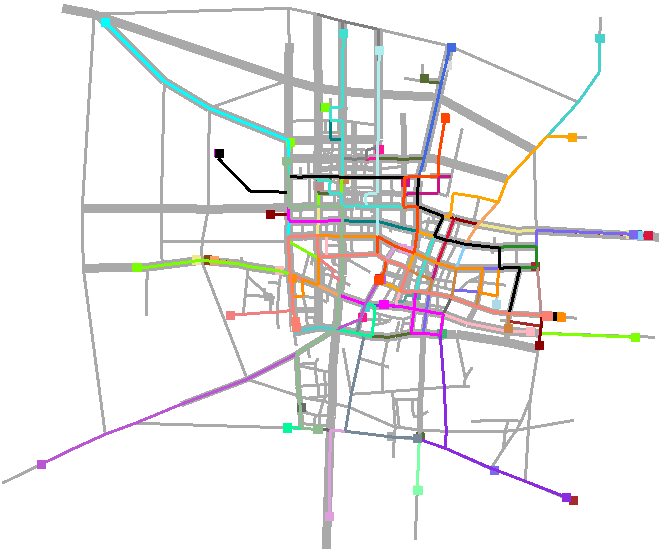
\includegraphics[width=0.8\textwidth, angle=0]{scenarios/figures/baoding_fig1.png}}%
{}
% ------------

% ------------
\createfigure%
{Performance comparison of scenario 1 and 2}%
{Performance comparison of scenario 1 and 2}%
{\label{fig:baoding_fig2}}%
{%
  \createsubfigure%
  {Car}%
  {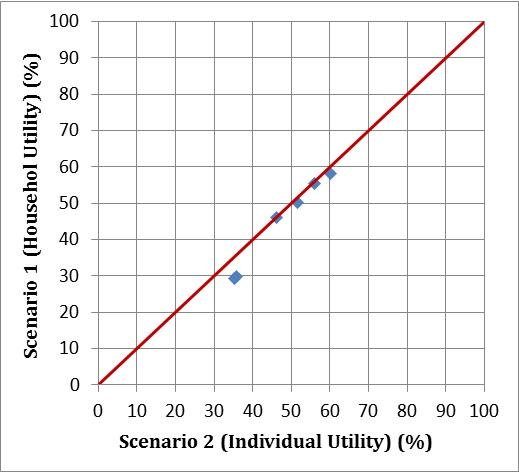
\includegraphics[width=0.7\textwidth,angle=0]{scenarios/figures/baoding_fig2a.png}}%
  {\label{fig:baoding_fig2a}}%
  {}%
  \createsubfigure%
  {Public transit}%
	{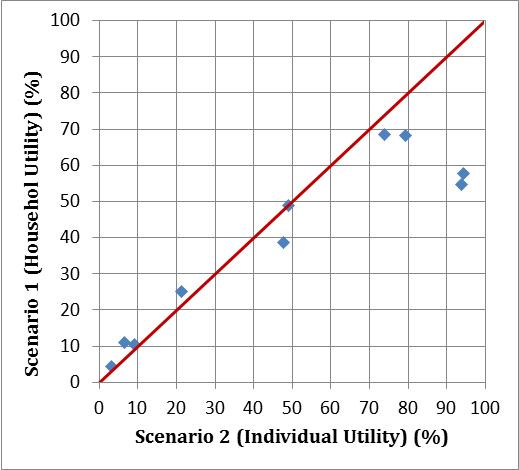
\includegraphics[width=0.7\textwidth,angle=0]{scenarios/figures/baoding_fig2b.png}}%
  {\label{fig:baoding_fig2b}}%
  {}%
}%
{}
% ------------

% ##################################################################################################################
